\chapter{Introducción}
\label{cap:introduccion}

Este documento recoge todos los aspectos fundamentales para comprender la funcionalidad de la aplicación web y móvil diseñadas como Trabajo de Fin de Grado para facilitar la gestión de \textit{stock} de ingredientes en restaurantes.

La idea del proyecto surge de la necesidad de una gestión rápida y eficiente a la hora de dirigir un restaurante, que son unas de las cualidades más importantes para llegar a conseguir un negocio de éxito.

Hasta hace poco tiempo en cualquier restaurante, la forma de llevar a cabo el trabajo se basaba en que el camarero tomase nota de lo que quería el cliente con una libreta y un bolígrafo, y se lo llevase a cocina para su preparación. Incluso podía el camarero decirte la típica expresión: "voy a consultar en cocina a ver si está disponible ese plato", aunque este tipo de gestión la podemos seguir viendo hoy en día en cualquier pueblo o chiringuito de playa.

Nos encontramos en una nueva era digital en la que se necesitan herramientas capaces de facilitar un trabajo eficiente, acotado en tiempo y con la calidad que esperan los clientes. La idea, por tanto, es acelerar al máximo los procesos de organización de un restaurante de manera que el gestor del restaurante pueda planificar y estructurar el servicio a los clientes, teniendo acceso a la configuración de diseño del menú del día, y los platos a elaborar.

En el mundo de la gastronomía el éxito se consigue a través de una buena materia prima, una buena puesta a punto en la elaboración de sus platos y una excelente atención al cliente con un servicio rápido y de calidad. En nuestro caso, nos hemos centrado en este último punto, reduciendo tareas manuales que consumen mucho tiempo haciendo más difícil concentrarse en la atención al cliente con un servicio de calidad.

Para conseguir este objetivo nuestro proyecto se centra, por una parte, en una comunicación dinámica entre cocina y empleados de sala, proporcionando una gestión rápida y eficaz a la hora de atender a los clientes y por otra, en facilitar una gestión sencilla de la administración del \textit{stock} de los ingredientes y productos.


\section{Objetivos}

El software desarrollado se centra en la mejora y optimización de la gestión del \textit{stock} y la comunicación entre camareros y cocina. Los objetivos serán, por tanto, la mejora de la eficiencia, la reducción del tiempo necesario y el aumento de la calidad del servicio a los clientes mediante un sistema automatizado de tareas combinado con una amplia base de datos donde almacenar toda la información y acceder a ella rápidamente.

La utilización de una aplicación web para la gestión y administración del restaurante asegura que los platos, bebidas o menús disponibles se ajusten exactamente a los ofertados al cliente y no haya errores entre los cocineros y los camareros. Además se permite acceso inmediato a la información de la base de datos con el objetivo de gestionar el \textit{stock} del restaurante. La actualización del \textit{stock} resultará, por tanto, extremadamente sencilla, ya que el gestor solo tendrá que reponer los ingredientes que estén por debajo de los niveles mínimos, para los cuales se genera una alerta para su reposición. Esto va a permitir dar una idea al gestor para la planificación de que platos elaborar en el menú de ese día.

Desde el punto de vista del trabajador, en este caso los camareros, la utilización de una aplicación móvil para la comunicación interna entre los trabajadores, asegura una comunicación directa con el cliente ofreciendo e informando los productos disponibles tanto en platos como en bebidas. De esta manera se genera un servicio rápido y de calidad a la hora de gestionar las comandas de cada mesa, sin generar esperas o preguntas en cocina que pueden disgustar al cliente.

Desde el punto de vista tecnológico, los objetivos que se plantean en este proyecto son los siguientes:

\begin{itemize}

\item Para la aplicación web, diseñar un software con una interfaz sencilla y que facilite el trabajo al gestor de la aplicación, como ver los ingredientes que han generado una alerta por estar por debajo de los niveles mínimos de \textit{stock} para una reposición de dichos ingredientes. Además, podrá generar un menú del día pudiendo seleccionar la cantidad de platos a elaborar para ese día, a partir de los ingredientes disponibles gestionando que platos se ofertaran de primero, de segundo y de postre.

\item Para la aplicación móvil, diseñar de la misma manera una interfaz sencilla y que facilite el trabajo a los trabajadores del restaurante, tanto a camareros como a cocineros. Podrán generar una comanda asignada a una mesa pudiendo tomar nota de las bebidas y los platos ofertados por la carta, además ofertar un menú del día tomando nota de los primeros y segundos platos, y del postre.

\item Diseñar una base de datos que permita el almacenamiento de una gran información, en la que guardaremos todos los ingredientes dados de alta en el restaurante, los platos con sus ingredientes asignados, las bebidas almacenadas o las mesas, cada una asignada con una comanda, y en cada comanda, almacenados los platos y bebidas pedidas por esa mesa.

\end{itemize}

\section{Plan de trabajo}

Teniendo en cuenta los objetivos descritos anteriormente, para el plan de trabajo se realizó una  estimación de tiempo con una duración de 7 meses. Para poder ver el plan de trabajo de una manera clara y sencilla decidimos hacer un diagrama de \textit{Gantt}.
El plan de trabajo se puede observar en la Figura~\ref{fig:Diagrama de Gantt} y la descripción de las actividades en la Figura~\ref{fig:Leyenda diagrama de Gantt}

\begin{figure}[h]
\centering
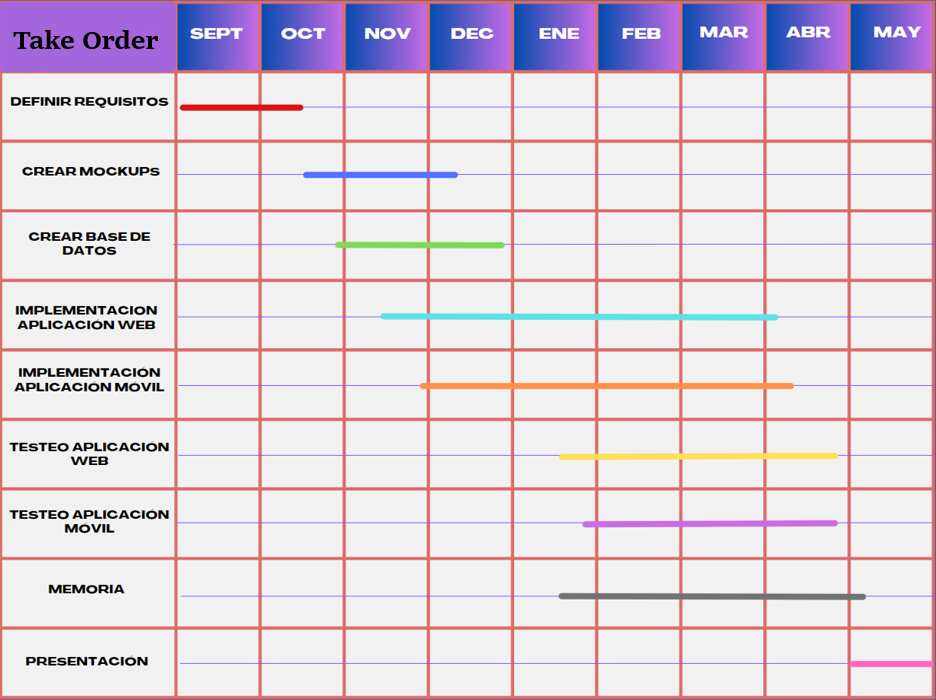
\includegraphics[width=15cm, height=11cm]{Imagenes/Figuras/Diagrama de Gantt.png}
\caption{Plan de proyecto}\label{fig:Diagrama de Gantt}
\end{figure} 


\begin{figure}[h]
\centering
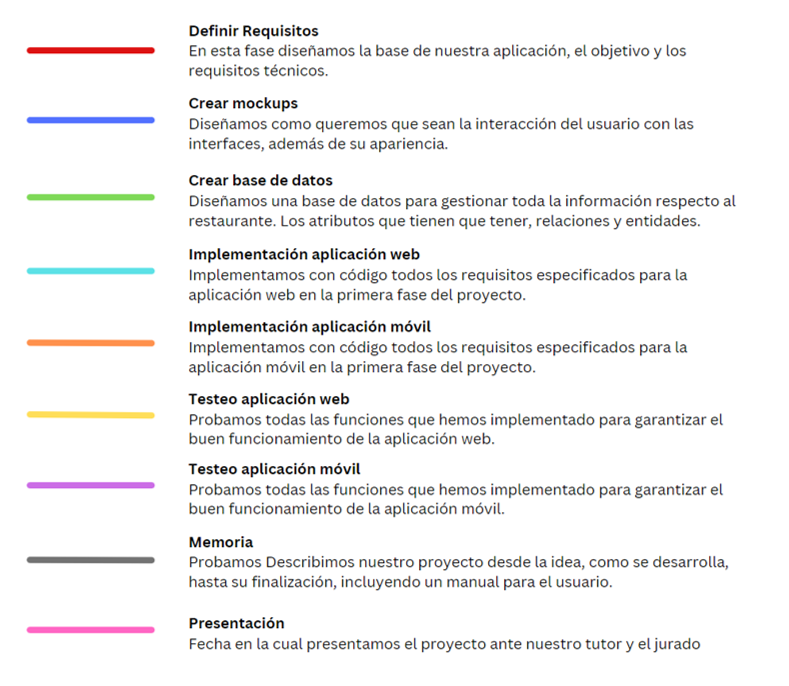
\includegraphics[width=15cm, height=12cm]{Imagenes/Figuras/leyenda Gantt.png}
\caption{Leyenda del plan de proyecto}\label{fig:Leyenda diagrama de Gantt}
\end{figure} 

